%f=linux; latex $f.tex; bibtex $f; latex $f.tex; latex $f.tex; dvips -t letter $f; ps2pdf $f.ps; evince $f.pdf
\documentclass{sig-alternate-05-2015}

%\usepackage{verbatim}
%\usepackage{comment}
\usepackage{epstopdf}

\newtheorem{observation}{\bf Observation}
\newtheorem{question}{\bf Question}


\begin{document}

% Copyright
\setcopyright{acmcopyright}
%\setcopyright{acmlicensed}
%\setcopyright{rightsretained}
%\setcopyright{usgov}
%\setcopyright{usgovmixed}
%\setcopyright{cagov}
%\setcopyright{cagovmixed}

\title{Code contribution practice in Linux kernel: 
How product structure shapes organization}

\numberofauthors{4}
\author{
\alignauthor
Ben Trovato\titlenote{Dr.~Trovato insisted his name be first.}\\
       \affaddr{Institute for Clarity in Documentation}\\
       \affaddr{1932 Wallamaloo Lane}\\
       \affaddr{Wallamaloo, New Zealand}\\
       \email{trovato@corporation.com}
% 2nd. author
\alignauthor
G.K.M. Tobin\titlenote{The secretary disavows
any knowledge of this author's actions.}\\
       \affaddr{Institute for Clarity in Documentation}\\
       \affaddr{P.O. Box 1212}\\
       \affaddr{Dublin, Ohio 43017-6221}\\
       \email{webmaster@marysville-ohio.com}
% 3rd. author
\alignauthor Lars Th{\o}rv{\"a}ld\titlenote{This author is the
one who did all the really hard work.}\\
       \affaddr{The Th{\o}rv{\"a}ld Group}\\
       \affaddr{1 Th{\o}rv{\"a}ld Circle}\\
       \affaddr{Hekla, Iceland}\\
       \email{larst@affiliation.org}
\and  % use '\and' if you need 'another row' of author names
% 4th. author
\alignauthor Lawrence P. Leipuner\\
       \affaddr{Brookhaven Laboratories}\\
       \affaddr{Brookhaven National Lab}\\
       \affaddr{P.O. Box 5000}\\
       \email{lleipuner@researchlabs.org}
}

\maketitle

\begin{abstract}

We investigate how the organization of contribution team and culture 
are affected by product/module structure in Linux kernel.
%and, in particular, if an inverse Conway's law holds: 
%``Developer culture for a legacy product mirrors the culture of organizations 
%that created and maintained that product in the past.'' 
In FLOSS projects, code commit privilege is often employed to ensure code quality.
Code committers are gatekeepers of code repository, and responsible for committing 
code for contributors who author the code but don't have the privilege to commit.
The ratio of number of authors over number of committers represents
how the contribution team is organized and suggests
a congruency of work load and communication in the team.
Different modules of Linux kernel present different structures, which
are associated with different business requirements
and different contributor activities.

Using code change history and developer interviews we investigate 
if the modules of Linux kernel with different structures have different
ratios and how they evolve in the diverse circumstances.
We find that 
%a) The product structure involves not just modules and cross-cutting concerns, 
%but also information retrieval strategies and other activity structure; 
a) Module structure has a dramatic effect on the organization of contribution
team (learning reproduces organization through product structure.).
In particular, the loose coupled (well modularized) modules like drivers would 
have a team size fluctuating at 20 (one committer works for 20 authors), and 
close coupled modules like kernel would have a size of 10.
b) The module structure is shaped by business requirements and 
contribution inflow.
c) Compact team tends to work together closely and have a shared control on code.  
On the contrary, loosely organized contribution team tends to work has stricter code ownership. 
We expect our findings could be used to improve FLOSS project 
contribution process by describing ways of organizing contribution teams
according to product structure characterized by features and contribution activities.
The findings also suggest that software teams maintaining 
legacy modules are likely to maintain the original (initial) culture 
and may be able to adjust to changing environment but with a delay.

\end{abstract}

\keywords{product structure, code commitment organization}

\section{Introduction}
%If I tell you to think of an open-source project, the first word that probably comes to mind is Linux. 

% 

Linux kernel has been a legend in the Free/Libre and Open Source Software (FLOSS) world.
Linux kernel based distributions (operating systems) established a commercial success
that many other FLOSS projects would like to pursue.
For example, they take 98.8\% positions in the top 500 fastest supercomputers 
in Nov 2015\footnote{https://en.wikipedia.org/wiki/Usage\_share\_of\_operating\_systems}.
The statistics from monitoring a substantial number of web sites during the 
last twelve months (until Dec 2015) show Linux kernel based
web clients have a 28.89\% share in the market.

The success of Linux kernel can not be achieved without the contributions
from participants. Starting from Linus Torvards,  volunteers
played a crucial role in the development of linux kernel. 
However, the number of volunteers (unpaid developers) contributing to the 
Linux kernel has been slowly declining for many years, now sitting at just 
 12.4\% (it was 13.6\% in 2014, and 14.6\% in 2013).
Meanwhile, commercial participation substantially grows in recent years,
large companies like RedHat and Intel put substantial resources on the development
of Linux kernel, e.g., Intel contributed 10.5\% of changes, ReHat 8.4\% 
in 2014\footnote{https://s3.amazonaws.com/storage.pardot.com/6342/120970/lf\_pub\_whowriteslinux2015.pdf}.
Now more than ever, the development of the Linux kernel is a matter for 
the professionals, as unpaid volunteer contributions to the project reached their 
lowest recorded levels in the latest ``Who Writes Linux''
report\footnote{http://linux.slashdot.org/story/15/02/18/1745246/torvalds-people-who-start-writing-kernel-code-get-hired-really-quickly}.

\begin{comment}
As for why Linux is now mostly developed by well-paid engineers, the 
possible reasons are myriad. The most obvious and compelling reason 
is that these big companies have a commercial interest in the continued 
good health of Linux. 10 years ago, Linux was the plaything of hobbyists 
and supercomputer makers -- today, it powers everything from smartphones 
(Android) to wireless routers to set-top boxes. The continuing commercial 
interest in Linux is highlighted by another statistic from The Linux 
Foundation report: In mid-2011, only 191 companies were involved in the 
Linux kernel; by the end of 2013, that number was up to 
243\footnote{www.extremetech.com/computing/175919-who-actually-develops-linux-the-answer-might-surprise-you}.
%If the Linux kernel was to survive, it would need new programmers to fix all of 
%the bugs that were added\footnote{eudyptula-challenge.org}.
\end{comment}

Apparently, Linux kernel experienced dramatic change since the very
beginning, e.g., expanding of substantial code and increasing of commercial participation.
Different modules of Linux kernel present different nature
and attract different contributors. For example, the module of drivers
accounts for the largest proportion of linecount (56.6\%) in the kernel, 
probably because various of 
hardware manufacturers have been trying to get their drivers into the kernel
and devoted substantial effort for their cause.
 As for the module of kernel, the very central one, attracting the most
capable and ambitious developers in the world, takes only 1.2\%.
According to Conway's law~\cite{conway}, the structure of software reflects 
the communication structure of people writing it.
It is of interest to understand how different modules present different
structure, whether or not that is associated with their contribution practice,
% contribution practice of different modules of Linux kernel differs from each other, 
and how they evolve over time adapting to different business environments. 
In particular, we aim to answer the following questions:
\begin{itemize}
\item What are the structures of different modules of Linux kernel?
\item Do different modules of Linux kernel have different contribution practice from each other?
\item Is there any relavance between module structures and contribution practice in Linux kernel?
%? \item Do different modules of Linux kernel evolve their practice over time and how?
%? participant feature: contribution type, and objective of contribution

\end{itemize}
On the one hand,
it may help us understand the new challenges in the new FLOSS landscape like
commercial participation.
On the other hand, the understanding can help us
utilize the best practices and amplify the effect. 

%In our study, the three aspects we investigate are all crucial for hybrid
%project development and the results of the measures we construct are agreed
%with reality, suggesting their validity.

%By using code change history, we quantify how contribution is organized for this FLOSS project.
We retrieve the code commits from the mainline repository of linux kernel, and 
use the data to quantify the community contribution practice.
We observed that module structure present ..........
We focus on one particular factor that tries to measure the team
relationship between code authors and code committers representing contribution
organization. We found the module of drivers is unique among all the modules 
in terms of having the biggest team size and organized more spontaneously. %code ownership?
We found the ratio
of number of authors over number of committers is decreasing over time for all the modules.
Even both the number of authors and committers are increasing (the module of 
drivers is the single module that has a sharp increase for both that is different
from the other modules), apparently, 
the increase of committers is faster than that of authors.
That may suggest a more professional organization of the working teams 
has been happening in the community.
Moreover, the ratio of each module correlates with the number of new joiners,
and the number of new LTCs. This may imply that a looser control of working team
brings more outsiders which requires attention from the community.

The rest of the paper is organized as follows. Section~\ref{s:related} 
discusses the related work. Section~\ref{s:method} describes the research 
methodology used in our study. Section~\ref{s:result} presents the results 
of our study. Section~\ref{s:limitation} discuses limitations of our study. 
We discuss practical implications of our empirical results in Section~\ref{s:discussion} 
and conclude in Section~\ref{s:conclusion}.

\section{Background and Related Work}\label{s:related}

%online communities can be designed and managed to achieve the goals that their owners, managers or members desire.~\cite{Kraut2012}
%Open source software development communities have the potential to provide firms with a valuable
%platform for innovation and product development (Chesbrough 2003). In order to realize such potential
%benefits, a firm must participate in an OSS community. If such involvement is articulated through direct
%contributions by the firm's developers, the firm has to choose which software developers to dedicate to
%this effort~\cite{Daniel2011}.
The nature and performance of FLOSS development are subject of
numerous investigations, but studies on evolution of contribution practice
along the change of project landscape particularly commercial participation
 are far less common.

An early study of Apache web server and Mozilla web browser~\cite{MFH02}
quantified various aspects of OSS development practices. The
results were framed as seven hypotheses that outline key aspects of
OSS development.  In this paper we focus on a different aspect of
 contribution organization. 

Community strategies and practices are often addressed in the
literature, e.g., community architecture~\cite{MFH02,YK03}, license
and intelligence property management mechanism~\cite{Hippel03}, and
code commit privilege or ownership control~\cite{MFH02,YK03,KSL03}, etc.
  Meneely  and  Williams~\cite{meneely09}  examined  the  relationship  
of  the  number  of  developers  working  on  parts  of  the
Linux kernel with security vulnerabilities.  They found
that when more than nine developers contribute to a source
file, it is sixteen times more likely to include a security vulnerability.

Unlike in prior work, we observe the contribution practice 
presented by Linux kernel experiencing various of technical and economic landscape 
and quantify the important aspects of the development that are likely 
to be affected by the product structure:
 the organization of author to committer team.

According to Conway's law~\cite{conway}, the structure of software reflects 
the communication structure of people writing it.
Conway's law emphasizes the effect on the artifacts induced by social activities, 
and provides insights on how to look at software development
through the perspectives of organizational science.

\section{Methodology}\label{s:method}
\subsection{Data preparation}
We retrieved all the commits from the mainline repository of Linux 
kernel\footnote{git://git.kernel.org/pub/scm/linux/kernel/git/torvalds/linux.git}.
We took steps to clean and standardize the data, and obtained
a data level for the further analysis.
Table~\ref{tab:data} shows an observation used for this study.
Each observation is a change committed to the mainline repository
maintained by Linus Torvalds. It records who and when writes the code,
and who and when commits the code, the author and the committer may be
the same person, but most of the time (74\%) they are not.
The changed file is represented by its directory in the code repository.
For example, ``drivers/pci/iova.c'' illustrates that the changed file
is under the directory of pci driver.

We use directory structure to measure 
We followed the following rules to obtain the final changes for this study.
1), we only look at c files.
2), we consider the first level modules retrieved from the file path 
as the module structure used in linux kernel. Overall we obtained 22 modules.
The top seven modules, in terms of number of changes, include drivers, arch, net, fs, sound, kernel, mm.
3), We consider a developer's joining time as the time they author their first commit.

\begin{table*}
\centering
\caption{Attributes of an observation}
\begin{tabular}{c|c|c|c|c|l} \hline
author & author time & committer & commit time & changed file & module\\ \hline
 Minfei Huang & Nov 6 16:32:45 2015 -0800 & Linus Torvalds & Nov 6 17:50:42 2015 -0800 & kernel/kexec.c &kernel\\ \hline
\label{tab:data}
\end{tabular}
\end{table*}

%\section{Module Structure and Metrics}

\section{Metrics}
%We measure three aspects of Linux kernel community to observe the evolution of its contribution practice.
\paragraph{Modularity}
% use entropy to measure modulization in a 3-year window
We use directory structure to measure modularity of one module. While defining modularity, we have three considerations: \\
1) one directory may have subdirectories, which means that one module may have submodules. Fox example, in Linux kernel, the $drivers$ directory has a sub directory named $staging$, 
which contains numerous subdirectories with many drivers. All of the contained drivers in $drivers/staging$ are drivers that need more development before being added to the mainstream kernel. Further, subdirectory may also have subdirectories, therefore we take\\
%+ need further explaination: smallest granularity.
2) modularity of one module may change over time, thus we take three years as a window, sliding month by month;\\
3) one module's submodules may differ greatly in terms of number of changes. For example, module A has two submodules with 10,000 and 100 changes respectively, and module B has two submodules with 10,000 and 10,000 changes respectively, then we will say module B has a higher degree of modularity than A.

Considering three aspects above, we have the definition of modularity of one module in a given period
\begin{equation}
\label{def_modularity}
M = \sum\limits_{i=1}^{N} - p_{i} \log p_{i}, 
\end{equation}
where $N$ is the number of submodules of the given module, and $p_{i}$ is defined by
\begin{equation}
\label{def_pi}
p_{i} = \frac{n_{i}}{\sum\limits_{i=1}^{N} n_{i}}, 
\end{equation}
where $n_{i}$ is the number of changes of the $i$th submodule.


\paragraph{Ratio of authors to committers}
We focus on one particular factor that tries to measure the team relationship between
code authors and code committers. Code authors in this study are people who
write the code that gets into the mainline repository. Code committers are
people who have the privilege to write the repository. A committer may be
responsible for a specific module (functionality), so responsible for committing
whoever's code on that module. 
%? subtle consideration: ratio of #A to #C --> load of cmtr ?
Naturally, the ratio of number of authors over number of committers may represent the load of a committer, or the difficulty (easiness) of the module, or, how hard it is for the author to 
get her code in. And the change of the ratio on the same module may represent
the change of project landscape (e.g., new features may attract more authors but
committers may keep at the same level as before), or the maturity of the module (e.g.,
a mature module may reduce committers). 

\paragraph{Code ownership}
%? define ownership: different from 'subsequent #athr of one file'
Ownership is a key aspect of large-scale software development,
 a valid proxy for expertise. Strong ownership, i.e., 
 a single key developer responsible for a particular component in a system (whether
it be a file, class, module, plugin, or subsystem), might be more
effective in carrying out all tasks consistently
and to completion~\cite{nordberg03}.
 Low communication overhead is required. External communications occur
through a single channel.
However, the disadvantages are obvious.
It might be necessary to trade overall development time for development
efficiency.  The system will have a low truck number -- only one developer 
need be hit by a truck to kill the project.
 Rogue individuals might ``own'' their code
to the exclusion of organizational goals.
It's common for commercial organizations to enforce strong code
ownership in order to achieve good quality, see, e.g., ~\cite{bird11}.
Given the informal, distributed way in which FLOSS projects like linux kernel are built, 
%we wanted to investigate whether some form of "code ownership" has evolved.
it seems that rather than
any single individual writing all the code for a given module, those in the core group
have a sufficient level of mutual trust that they contribute code to various modules as
needed~\cite{MFH02}. In FLOSS projects, code "ownership" to be
more a matter of recognition of expertise than one of strictly enforced ability to make
commits to partitions of the code base.

One measure of ownership
is how much  of  the  development  activity  for  a  component
comes from one developer. If one developer makes 80\% of
the changes to a component, then we say that the component has high 
ownership. 

  The proportion of ownership  (or  simply  ownership)  of  a  contributor  for  a
particular component is the ratio of number of commits that the contributor has made 
relative to the total number of commits for that component.  Thus, if
Cindy has made 20 commits to ie9.dll and there are
a total of 100 commits to ie9.dll then Cindy has an ownership of 20\%.

%A concept of \emph{``OSS governance''} is used to describe the way
%the OSS communities achieve direction and coordination~\cite{Markus07}.
%OSS governance can be defined as the means
%of achieving the direction, control, and coordination of wholly or partially
%autonomous individuals and organizations on behalf of an OSS development project
%to which they jointly contribute.

%Bonaccorsi et al.~\cite{Bonaccorsi06} found that many firms 
%follow a hybrid business model by mixing products, types 
%of licenses, and sources of revenues.
%They developed a measure of the degree of
%openness to open source and built a model of determinant factors.
%They found that switching costs on the supply side and network externality 
%effects on the demand side negatively influence the degree of openness.

\section{Results}\label{s:result}


\subsection{Module Structure}
We have observed two aspects of product structure: the architecture, 
which includes several structures, of which we will primarily focus 
on the module structure, and the development activity structure. 

Based on our interviews and prior experience, developers' tasks are 
assigned based on these two types of structure. In our study the 
module structure was organized according to product package/subsystem 
and functionality (functionality, such as internationalization, may cut 
across the package/subsystem boundaries). 

The activity structure followed common development practices, such as 
building, installing, configuring, and testing the product. It also 
included practices used to fix and report problems and to design and 
develop new features. Furthermore, underlying these generic practices, 
there were substantial differences in information seeking behavior needed 
to accomplish these common tasks, for example, knowing when and how to 
inspect the execution log or where to find information about similar bugs 
that occurred in the past, and variation in acceptable norms, such as how 
many defects are acceptable, and what should be tested, how it should be 
tested, and how extensively it should be tested. 

Based on our observations, the way each practice was implemented was carried 
over from the original practice used to develop the products, often with no 
individuals serving as conduits. For example, when fixing defects Project A 
extensively used their rich problem resolution repositories, while project C 
used almost exclusively the logs of product execution and project B focused 
on latest code changes. 

Our claim is not that the mere fact that the original team and the new team 
perform testing implies some learning from the product structure (we expect 
that most software developers know about testing from their undergraduate 
studies). Rather, the similarity between the ways testing was done in the 
original and the new team indicates that the product itself has some effect 
on learning and that product structure incorporates development activity 
structure.
We propose that developers learn through performing regular project tasks 
under the constraints (``guidance'') of the product structure, and, accordingly, 
change their positions in the project/organization. The centrality of a task, 
embodies the centrality of the modules or activities the task is related to, 
and reflects the centrality of the position the developer has in the 
organizational communication.


%ratio of authors to committers --, 除了net, 基本都在减小, why? 协作成本越来越高么?
\subsection{Organization of Code Contribution} %{Ratio of authors to committers}
we focus on one factor that tries to measure the team relationship between
code authors and code committers. Code authors in this study are people who
write the code that gets into the mainline repository. Code committers are
people who have the privilege to write the repository. A committer may be
responsible for a specific module (functionality), so responsible for committing
whoever's code on that module. 
Naturally, the ratio
of number of authors over number of committers may represent the load of a committer,
or the difficulty (easiness) of the module, or, how hard it is for the author to 
get her code in. And the change of the ratio on the same module may represent
the change of project landscape (e.g., new features may attract more authors but
committers may keep at the same level as before), or the maturity of the module (e.g.,
a mature module may reduce committers). 

We use this measure to investigate how 
the code contribution is organized and how the balance
between authors and committers is achieved in the community.
We take three years as a window, start from January 2005 (the window
is from January 2005 to December 2007) and roll the window by month until the window
getting to December 2015, i.e., the date we retrieved the data.
We calculate the metrics on these windows.
Considering the variations of the modules, we look at the team organization
on each module separately.
Figure~\ref{fig:atr2cmtr} presents the ratio changes in a three-year window
rolling from January 2005 month by month.

Overall, the ratio is decreasing over the years.
Even both the number of authors and committers are increasing (drivers is
the single module that has the sharpest increase for both), apparently, the
increase of committers is faster than that of authors.
That may suggest a more professional organization of the working teams 
has been happening in the community.

As we can see, the module of drivers (the top line) has a much higher ratio 
than the other modules. It fluctuates at around 20 compared to 10 that the
other modules move around.
If we look at the number of authors and committers separately on the modules, 
we can see that they both grow over time on all the modules, but the drivers 
module has the biggest growth. At the same time, even both authors and committers
 grow, apparently committers have a slower growth, therefore the ratio drops.

We discovered that the ratio is around 10 for most modules but high above 10 for
the module of drivers. 
The ratio for modules like kernel, mm stabilizes at 6 or 7, a reasonable % a reference for team size 7?
size that is a controllable number for a team.
A further investigation reveals that the drivers module have a much looser control over
the team, the fact that a committer works for 20 authors suggests that the tasks 
may be easy on this feature. Net drivers and staging drivers appear to be on
the easiest tasks, suggesting a place where newbies like to start. The fact
that the drivers module has more than 50\% share of newcomers supports this
hypothesis (what's the proportion of changes of drivers?).
In fact more than 40\% of all the committers in the kernel community
started from the drivers module (no comitters of kernel module or mm module started from kernel or mm).

We take a further investigation to understand the story in the module of
drivers. Figure~\ref{fig:ratiodrivers} shows the ratios of subdirectories under the
drivers.  We can see net, staging and media are the three sub-modules that
are different from the others that have the similar trend compared to the
modules at the first level, i.e., they fluctuate at 10.

The investigation on net module shows 10 is a common number for this metric,
as presented in Figure~\ref{fig:rationet}.
Actually except mac80211, all the other sub-modules fluctuates at 10 (sunrpc
seats at five).  A closer look at mac80211 clarifies its change:
the number of committers is from 3 to 8 and back to 3, but the number of
authors stays the same, making the curve change sharply.

\begin{figure}
\centering
\includegraphics[height=2.33in, width=3.5in]{./pics/a2c-in-mod.pdf}
\caption{Ratio of \#authors to \#committers}
\label{fig:atr2cmtr}
\end{figure}

\begin{figure}
\centering
\includegraphics[height=2.33in, width=3.5in]{./pics/testSmall.pdf}
\caption{Ratio of \#authors to \#committers on Drivers}
\label{fig:ratiodrivers}
\end{figure}

\begin{figure}
\centering
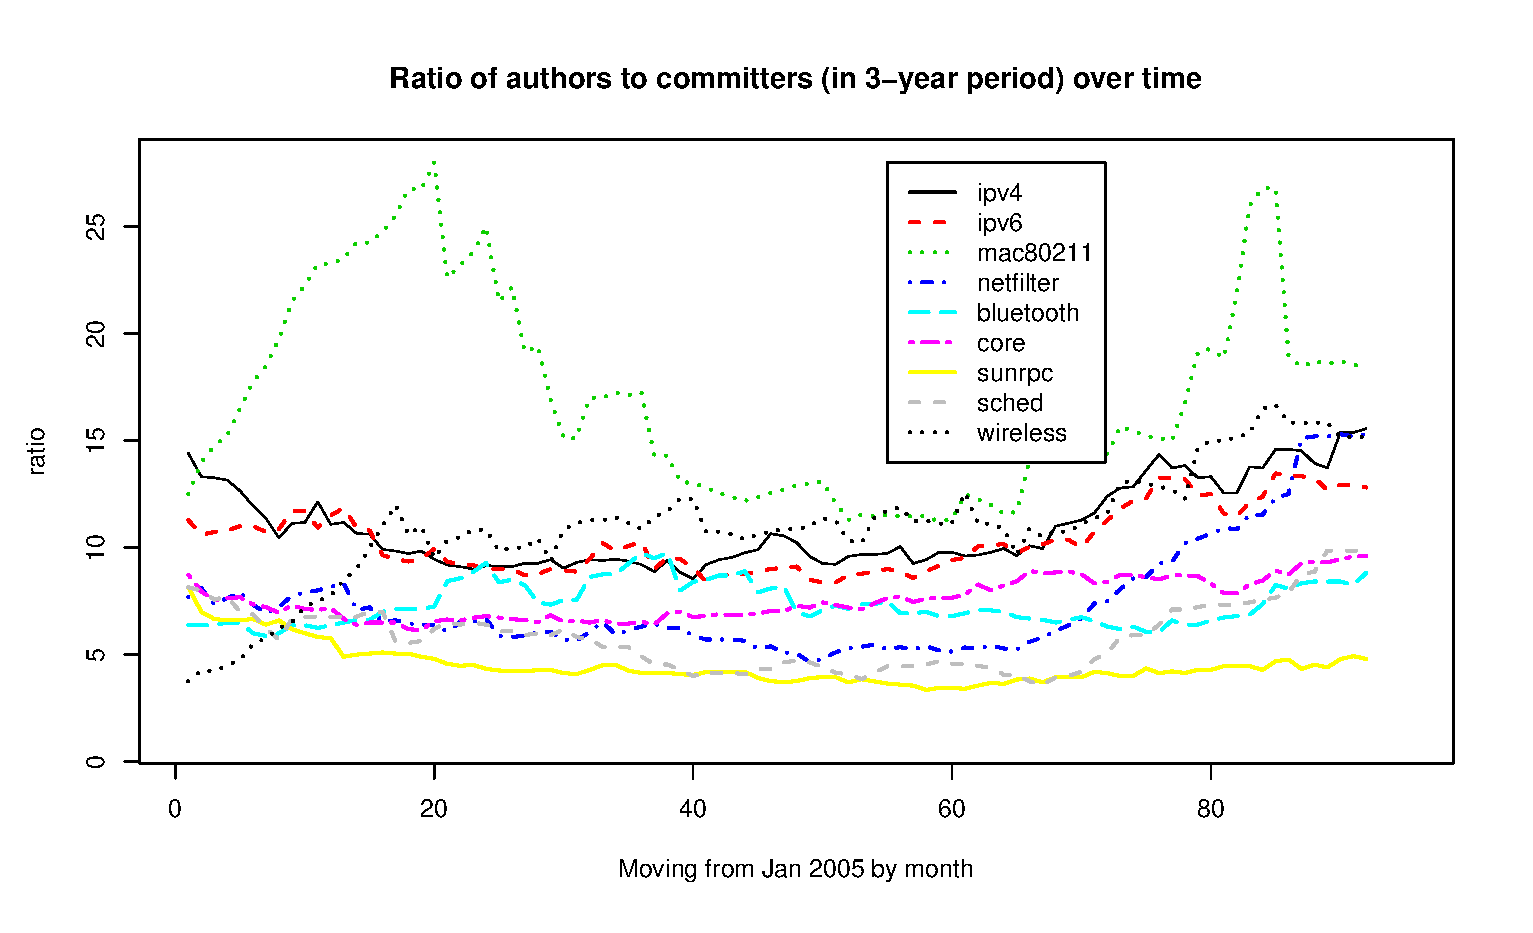
\includegraphics[height=2.33in, width=3.5in]{./pics/atr2cmtrNET.eps}
\caption{Ratio of \#authors to \#committers on Net}
\label{fig:rationet}
\end{figure}

In summary, 10 might be a reasonable number for organizing the contribution
team. If the code is well modularized, the ratio could be bigger, otherwise
it could be smaller.

Through chcking with the core members of kernel, we found the ratio changes because of the following reasons: \\
We use directory structure to measure 
1), when there is new feature, a bulk of authors would cause fluctuation of this measure,
because the committers wouldn't increase at the moment, e.g., drivers/staging/iio. \\
2), when there is new feature, the increase of committers is likely to be behind
the increase of authors, e.g., net/wireless, drivers/staging/comedi, drivers/staging/iio.  \\
3), for the matured feature, it's likely the committer would leave, and a small amount
of leaving committers would lead to a drama increase of this ratio because the proportion
is relatively high, e.g. net/mac80211. \\
4), in general the development is stable.

In summary, we have the following observation:
\begin{observation}\label{o:1}
 The suitable way of organizing code contribution team in Linux kernel is
to have a committer work for ten authors. If the code is well modularized, 
the ratio could be bigger, otherwise it could be smaller.
\end{observation}

The ratio for modules like kernel, mm stabilizes at 6 or 7, a reasonable % a reference for team size 7?
size that is a controllable number for a team.
A further investigation reveals that the drivers module have a much looser control over
the team, the fact that a committer works for 20 authors suggests that the tasks 
may be easy on this feature. Net drivers and staging drivers appear to be on
the easiest tasks, suggesting a place where newbies like to start. The fact
that the drivers module has more than 50\% share of newcomers supports this
hypothesis (what's the proportion of changes of drivers?).
In fact more than 40\% of all the committers in the kernel community
started from the drivers module (no comitters of kernel module or mm module started from kernel or mm).

\subsection{Code Ownership}
 The kernel which forms the core of the Linux system is the result 
of one of the largest cooperative software
projects ever attempted~\cite{kerneldvp}.
With the 2.6.x series (Linux 2.6.0 Released 18 December, 2003), the Linux kernel has moved to a relatively 
strict,  time-based  release  model. 
The stricter code ownership may be developed to simplify the cooperation
in the building of more and more complicated kernel.
However, we can still see the differences among different modules.

%Commercial involvement may bring an organized structure to the
%development process in addition to dedicating employees' time 
%to find and report issues.  In particular, companies might encourage
%stronger code ownership in contrast to loose code ownership observed
%in Apache and Mozilla projects~\cite{MFH02}.
The close coupled module is associated with close team, and we hypothesize 
that the close team are more likely to have shared code ownership in contrast
to the loose team.

Stricter code ownership would manifest itself as a smaller number of
developers changing a single file. The average number of changers
per file ($Changer_{avg}$) may, therefore, be used to measure the
strictness of code ownership. We calculated $Changer_{avg}$ for each
month of each module and the resulting time series of this measure of code
ownership are shown in Figure~\ref{fig:ownership}. 
We can see the modules of drivers and arch have a much stricter
ownership as compared to the other modules.
The module of kernel has the loosest control, next to it is the module of mm. 

\begin{figure}
\centering
\includegraphics[height=2.1in, width=3.5in]{./pics/avgchgerfileonmod(b).eps}
\caption{Code ownership of different modules}
\label{fig:ownership}
\end{figure}

The boxplot in Figure~\ref{fig:ownershipkernel} and Figure~\ref{fig:ownershipdrivers}
show a clear comparison between the modules of kernel and drivers.
(every boxplot has 12 numbers for every year) shows a clearer trend\footnote {The lower and
  upper boundaries of the rectangle of the box-plot represent the
  first and the third quartile and the thick line is the median. The
  lowest and upper horizontal lines represent the 1.5 quartiles away
  from the mean. The points below or above the horizontal lines are
  suspected outliers.}.
For example, in 2005 when drivers has a code ownership of 1.36 being the median, 
kernel has 2.62, almost twice of that of drivers.
In 2015 drivers has 1.50 and kernel has 2.89.
This is an indication that close team has a closer relationship on
sharing code.
% A suitable regression model
%shows that these observed decreases are significant for both projects. 

\begin{figure}
\centering
\includegraphics[height=2.1in, width=3.5in]{./pics/chgerfkernel.eps} %10*6
\caption{Boxplot of code ownership of kernel module}
\label{fig:ownershipkernel}
\end{figure}

\begin{figure}
\centering
\includegraphics[height=2.1in, width=3.5in]{./pics/chgerfdrivers.eps} %10*6
\caption{Boxplot of code ownership of drivers module}
\label{fig:ownershipdrivers}
\end{figure}

At the same time, we found the average number of unique files touched 
by a developer (per month) on different modules differ from each other
with a similar pattern. Figure~\ref{fig:fdvprkernel} and
Figure~\ref{fig:fdvprdrivers.eps} show the numbers of kernel and drivers
respectively, as we can see, developers of kernel module tend to touch
more different file as compared to developers of drivers module.
The number fluctuates around 10 for kernel module, but 5 for drivers module.
This may indicate that the sharing ownership brings more chances for
the expertise diversity.
On the contrary, for modules like drivers,
 it may require more effort to work on multiple files,
and the interconnections between files may be reduced in order to reduce
the needs of cooperations.
Developers need to put more effort on single files
instead of working with others on the same files.
This indicates a possible phenomenon that requires attention from the kernel community:
if people start to work on their own, there is a risk that the cooperation critical
for the health of the community is reduced.


\begin{figure}
\centering
\includegraphics[height=2.1in, width=3.5in]{./pics/fdvprkernel.eps} %10*6
\caption{Number of files touched by a developer each month on kernel}
\label{fig:productivitykernel}
\end{figure}

\begin{figure}
\centering
\includegraphics[height=2.1in, width=3.5in]{./pics/fdvprdrivers.eps} %10*6
\caption{Number of files touched by a developer each month on drivers}
\label{fig:productivitydrivers}
\end{figure}

%(code ownership更加intense, 以减少彼此合作的需要)
In summary, we have the following observation:
\begin{observation}\label{o:2}
\emph{The developers working on different modules present different extent of control
on the code. In particular, more structured modules have stricter code ownership
and compact modules are more likely to share the ownership.} 
\end{observation}

Moreover, the ratio of each module correlates with the number of new joiners,
and the number of new LTCs. This may imply that a looser control of working team
brings more outsiders.

\section{Discussion}\label{s:discussion}

\section{Limitation}\label{s:limitation}

\section{Conclusion}\label{s:conclusion}

\bibliographystyle{abbrv}
\bibliography{../paper/bib/audris,../paper/bib/all,../paper/bib/pkuas,../paper/bib/hybrid} 


\end{document}
